\documentclass[12pt,a4paper]{report}
\usepackage{siunitx}
\usepackage{amsmath}
\usepackage{amsfonts}
\usepackage{amssymb}
\usepackage[bottom]{footmisc}
\usepackage{verbatim}
\usepackage{graphicx}
\usepackage[utf8]{inputenc}
\usepackage[english]{babel}
\usepackage[left=3cm,right=3cm,top=2cm,bottom=3cm]{geometry}
%\usepackage[small,compact]{titlesec}
\usepackage{setspace}
\usepackage{hyperref,cleveref}
\usepackage{cite}
\usepackage{color}
\usepackage{palatino}
\usepackage{soul,xcolor}
%\usepackage{tikz}
\usepackage{caption}
\usepackage{subcaption}
\usepackage{siunitx}
\usepackage{url}
\usepackage{gensymb}
\usepackage{geometry}
\usepackage{upgreek}
\usepackage[square,sort&compress]{natbib}
\usepackage{datetime}
%\input{defs}

% Colors for links
\newcommand\myshade{85}
\colorlet{mylinkcolor}{blue}
\colorlet{mycitecolor}{orange}
\colorlet{myurlcolor}{red}
\hypersetup{
	linkcolor  = mylinkcolor!\myshade!black,
	citecolor  = mycitecolor!\myshade!black,
	urlcolor   = myurlcolor!\myshade!black,
	colorlinks = true,
}
% Color for strikethrough text
\setstcolor{red}

% Define stuff here
\def\albatros{ALBATROS}
\def\prizm{PRI$^{\rm Z}$M}
\newcommand{\attention}[1]{\textcolor{red}{\bf {#1}}}

\newcommand{\ieee}{Institute of Electrical and Electronics Engineers}
\newcommand{\aap}{Astronomy and Astrophysics}
\newcommand{\aaps}{Astronomy and Astrophysics Supplements}
\newcommand{\aj}{Astronomical Journal}
\newcommand{\apj}{Astrophysical Journal}
\newcommand{\jgr}{Journal of Geophysical Research}
\newcommand{\mnras}{Monthly Notices of the Royal Astronomical Society}
\newcommand{\nar}{New Astronomy Reviews}
\newcommand{\pasa}{Publications of the Astronomical Society of Australia}
\newcommand{\pasp}{Proceedings of the Astronomical Society of the Pacific}
\newcommand{\prd}{Physical Review D}
\newcommand{\prl}{Physical Review Letters}
\newcommand{\araa}{Annual Review of Astronomy and Astrophysics}
\newcommand{\apjl}{The Astrophysical Journal Letters }
\newcommand{\apjs}{The Astrophysical Journal Supplement Series}
\newcommand{\physrep}{Physical Reports}
\newcommand{\jrasc}{Journal of the Royal Astronomical Society of Canada}
\newcommand{\nat}{Nature Journal}
\newcommand{\ea}{Experimental Astronomy}
\newdateformat{monthyeardate}{%
	\monthname[\THEMONTH], \THEYEAR}


\begin{document}
	\begin{titlepage}
		
		\newcommand{\HRule}{\rule{\linewidth}{0.5mm}} % Defines a new command for the horizontal lines, change thickness here
		
		\begin{center}
			\begin{figure}[ht]
				\centering
				\includegraphics[width=0.7\textwidth]{Figures/UKZNLOGO.png}\\[1cm]
			\end{figure}
			
			\LARGE {\textbf {Low-Frequency Observations of the Radio\\[0.3cm Sky from Marion Island]}}\\[1cm]
			{By}\\[0.5cm]
			\textbf {\Large {Tankiso H. Moso}}\\[0.5cm]
			{\small Submitted in the School of Mathematics, Statistics and Computer Sciences\\in  fulfilment of the academic requirements for the\\Master of Science Degree in Applied Mathematics\\at the\\University of Kwa-Zulu Natal, Westville Campus}\\[3cm]
			
			\begin{minipage}{0.45\textwidth}
				\begin{flushleft} \large
					\hrulefill\\
					Supervisor Signature \\
					Prof. H. C. Chiang % Supervisor's Name
				\end{flushleft}
			\end{minipage}
			~
			\begin{minipage}{0.45\textwidth}
				\begin{flushright} \large
					\hrulefill\\
					Co-Supervisor Signature \\
					Prof. K. Moodley % Supervisor's Name
				\end{flushright}
			\end{minipage}\\[3cm]
			~
			\begin{minipage}{0.5\textwidth}
				\begin{center} \large
					\hrulefill\\
					Student Signature\\
					Tankiso H. Moso % Your name
				\end{center}
			\end{minipage}\\[2cm]
			
			{\large \monthyeardate\today}\\ % Date, change the \today to a set date if you want to be precise
		\end{center}
		
		
	\end{titlepage}
	
	\pagenumbering{roman}
	
	\addcontentsline{toc}{section}{Declaration}
	\section*{Declaration - Plagiarism}
	
	I, Tankiso H. Moso, declare that
	
	\begin{enumerate}
		\item The research reported in this thesis, except where otherwise indicated, is my original research.
		\item This thesis has not been submitted for any degree or examination at any other university.
		\item This thesis does not contain the data, photographs, graphs, or other material of other persons unless expressly recognized as obtained from other people.
		\item This thesis does not contain other persons' writing unless expressly recognized as having been sourced from other researchers. Where additional written sources have been cited, then:
		\begin{enumerate}
			\item Their words have been re-written, but the general information attributed to them has been referenced.
			\item Where their exact words have been used, then their writing has been placed in italics and inside quotation marks and referenced.
		\end{enumerate}
		
		\item This thesis does not contain text, graphics or tables copied and pasted from the internet unless specifically acknowledged, and the source being detailed in the thesis and the Bibliography section.
	\end{enumerate}
	\vspace{2cm}
	
	\begin{minipage}{0.5\textwidth}
		\begin{center} \large
			\hrulefill\\
			Tankiso H. Moso\\[1cm]
			
			{\large \today} % Date, change the \today to a set date if you want to be precise %Change the date to your date of submission
		\end{center}
	\end{minipage}\\[2cm]	
	
	\newpage
	\addcontentsline{toc}{section}{Publication List}
	\addcontentsline{toc}{section}{Publication List}
\section*{Publication List}

Publications arising from the work presented in this thesis:

\begin{enumerate}
	\item The Array of Long Baseline Antennas for Taking Radio Observations from the Sub-Antarctic~\citep{2020arXiv200812208C}, and 
	\item Radio-Frequency Interference at the McGill Arctic Research Station~\citep{2020arXiv201206521D} has been submitted.
\end{enumerate}




	
	\newpage
	\addcontentsline{toc}{section}{Abstract}
	\section*{Abstract}
	
Measurements of the radio sky at frequencies below \SI{\sim 100}{\mega \hertz} have the potential to unlock a new observational window into the universe’s history. These observations allow us to probe even earlier epochs of the universe’s history and lay the groundwork for eventually exploring the “dark ages” through to the cosmic dawn. There is minimal knowledge about the radio sky below \SI{30}{\mega \hertz}. The lowest measured frequency of the radio sky dates from the 1960s when Grote Reber mapped a portion of the sky at \SI{\sim 2}{\mega \hertz} using a 192-element dipole array with $\sim$5 \degree resolution. This brief glimpse of low-frequency Galactic emission was made possible partly by an unusually deep solar minimum.

This thesis presents the Array of Long Baseline Antennas for Taking Radio Observations from the Sub-Antarctic (\albatros) and upgrades to Probing Radio Intensity at high-Z from Marion (\prizm) subsystems. The two experiments are installed in Marion Island located in the southern Indian Ocean.  This thesis focuses on the deployment of the first autonomous \albatros\ station, which took place in 2019. Prior to the deployment of the autonomous station, the two-element pathfinder was installed to assess the observable frequencies from Marion below \SI{30}{\mega \hertz}. The final \albatros\ array will consist of ten autonomous antenna stations separated by maximum baseline lengths of \SI{\sim {20}}{km}. This thesis also presents the design of a new second stage electronics (SSE) enclosure and other subsystem upgrades for \prizm\ that were intended for the 2020 deployment. The enclosure was revised so that each antenna is serviced by its SSE box and more compact subsystems were designed to fit in the new box.

Preliminary observations from the \albatros\ pathfinder installed in April 2018 show discernible interferometric fringes from the sky visible down to \SI{\sim 10}{\mega \hertz} without any data processing or cuts. The first fully autonomous antenna station was deployed in April 2019, configured to record baseband data, and with power supplied by solar panels. The first autonomous \albatros\ station is fully operational. The solar power system sufficiently charges the batteries, the hardware was successfully secured against the wind storms and mice, and the preliminary low-frequency data are exceptional compared to the pathfinder observations as we are currently experiencing a solar minimum. So far, the new solar power control electronics appear to be radio-quiet and there is no qualitative evidence of self-generated contamination from radio-frequency noise.

	
	\newpage
	\addcontentsline{toc}{section}{Acknowledgements}
	\section*{Acknowledgements}

Throughout my life, I have been blessed, highly favored, and fortunate to have been granted several opportunities that have led me to undertake this research thesis. Thank you to the thousands of people in the universe who have provided me with the foundation, environment, safety, health, support, service, financial well-being, love, joy, knowledge, kindness, calmness, and happiness to produce this work.

My sincerest gratitude goes to Profs. Cynthia Chiang and Jonathan Sievers for giving me a platform to realize and prove my strengths and capabilities. The unusual path that I took in joining radio astronomy research is a lifetime opportunity that has opened doors for me and my career. Words can never express my gratitude for the life skills, adventurous experiences, and independence that I have gained through you. It has indeed been a great ride!

I want to thank Prof. Matt Hilton and Dr. Ilya Sinayskiy. During the years that I have spent at the University of KwaZulu Natal, you have had a remarkable impact on my academic and career growth and recognition. 

A special thanks to the National Astrophysics and Space Science Programme for funding my studies since 2018. This thesis's completion would not have been possible without collaborative efforts from the McGill University, \prizm\ and \albatros\ teams, and the H1-225 lab mates. 

All my friends and acquaintances who have been pushing me to do and be the best I can, I thank you all for therapeutic sessions, academic, financial, personal growth, empathy, motivation, and outings.

My family's prayers throughout this journey of life have been my greatest pillar of strength. The support I receive from you, Mongi is immeasurable; thank you for always having my back. \\[4 cm]


\begin{center}
	\emph{"Dear God, thank you...!"}
\end{center}



	
	\newpage
	\renewcommand\contentsname{Table of Contents} %This changes the original latex contents name to 'Table of Contents'
	\tableofcontents\newpage %This adds the table of contents to your thesis.
	
	\pagenumbering{arabic}	
	
	\chapter{Introduction}

Our Universe's origin has always been a mystery until such time, when humankind started looking for answers to the unanswered questions about the evolution of the cosmos. The search for solutions led to a field of study called cosmology. This field has drastically impacted our knowledge of the universe's evolution~\citep{book:909085}.

Humans initially believed that the Sun, the moon, and other planets orbited the Earth until Nicolaus Copernicus and other astronomers replaced the geocentric model with the heliocentric model~\citep{sep-copernicus, kanas}.  Celestial mechanics emerged as an area of study after Isaac Newton discovered that elliptical planet motion can be explained by gravitational force attraction~\citep{crowe2013theories,sep-copernicus}. In the modern study of the Universe, our understanding of gravity has been further refined by Albert Einstein's theory of general relativity, which presents the mathematical framework required to describe the evolution of the universe.
	
As a result of all these findings \attention{[you haven't discussed ``these findings'' yet---discuss the discovery of the expanding universe and the CMB first, before introducing the big bang model]}, Georges Lemaitre proposed the Big Bang theory, the contemporary model that provides a complete explanation of the Universe expansion~\citep{1926ApJ....64..321H}. The Big Bang theory was established from Hubble's law and subsequently by Arno Penzias and Robert Wilson in 1964 from discovering the cosmic microwave background (CMB)~\citep{1965ApJ...142..419P,2003RvMP...75..559P,1929PNAS...15..168H}. The Supernova Cosmology Project and the High-Z Supernovae Search Team in 1998 discovered the acceleration of the Universe using observations of type Ia supernovae~\citep{1998AJ....116.1009R, 1999ApJ...517..565P}. The accelerated expansion is described by dark energy, which accounts for approximately 74 percent of the Universe's energy density. Today, understanding the nature of dark energy is a major area of focus in astrophysics and particle physics~\citep{2008ARA&A..46..385F}. 
	
	\section{History of the Universe}
	
	\autoref{Fig:timeline} shows the cosmic history of the Universe. The Planck era, which lasted unil \SI{e-43}{s} after the big bang is unknown to physicists and requires a quantum theory of gravity. Following the Planck era, \SI{e-34}{s} after the big bang, the universe went through a period of rapid exponential expansion, known as Inflation~\citep{1981PhRvD..23..347G}.

	\begin{figure}
		\begin{center}
			\includegraphics[width=\linewidth]{Figures/Reionizationtimeline.jpg}
			\caption{The cosmic history of the Universe from the Big Bang to its early years, through the dark ages to the epoch of reionization and the post-reionization epoch. Image credit:National Optical Astronomy Observatory}
			\label{Fig:timeline}
		\end{center}
	\end{figure}
        
	Recombination occurred when the universe cooled enough for neutral hydrogen (HI) to form, around a redshift of $z$ $\sim1100$. The redshift-wavelength relation is \attention{[include a brief phrase here describing what redshift physically means, i.e. that higher redshift means earlier times] given} by
	\begin{equation}
	\begin{split}
	1+z & = \frac{\lambda_{obs}}{\lambda_{emit}}= \frac{1}{a}
	\end{split}
	\end{equation}
	where $z$ is the redshift, $\lambda_{obs}$ is the wavelength of the observed signal, $\lambda_{emit}$ is the wavelength of the signal emitted, and $a$ is the Universe expansion scale factor. Prior to recombination, electrons were not bound to protons, and the Universe contained ionized plasma known as photon-baryon fluid. Decoupled photons then formed the CMB~\citep{1965ApJ...142..419P}.

	Subsequently, HI became the dominant baryonic component of the intergalactic medium (IGM) during the dark ages ($1100 \gtrsim z \gtrsim 30$). No measurements of the dark ages exist, and if hydrogen can be mapped in this era, valuable cosmological data can be produced~\citep{11, 2004PhRvL..92u1301L}.
	
	There were density fluctuations in the distribution of matter, and the overdense regions collapsed under the influence of gravity, ultimately creating the first stars. Thus, nuclear reaction resulted in Cosmic Dawn ($30\gtrsim z \gtrsim 10$). Energy from the first stars ultimately fully reionized the Universe. Galaxies, galaxy clusters and large-scale structures that exist in the present universe evolved after the first stars were born~\citep{2017arXiv170808521D, 2012AdSpR..49..433B}. 
	
	Throughout the cosmological epochs, what is known is minimal because it is challenging to observe them directly. The growth of \SI{21}{cm} cosmology has the capability to fill the gaps in our knowledge of the universe's history~\citep{2012RPPh...75h6901P}. A brief overview of the history of the Universe has been given, and the next section will cover 21 cm cosmology corresponding to the dark ages and cosmic dawn in more detail.
	           
	\section{Cosmology with Redshifted 21-cm Emission}
		
	Because hydrogen gas is the most abundant element in the universe, there is a concerted effort in the experimental community to develop telescopes for mapping neutral hydrogen via \SI{21}{cm} emission. This hydrogen line is an essential mechanism for probing the dark ages to the epoch of reionization (EoR)~\citep{2013PhRvD..87d3002L,2014ApJ...782...66P}. The generation of the hydrogen line (\SI{21}{cm} line or HI line) is due to the intrinsic spins of the electron and proton within the hydrogen atoms~\citep{book:832129}. The electron and proton spins can be oriented in either the opposing or the same direction respective to each other. When the spins are opposing or antiparallel, the hydrogen atom is in the lower energy state. When the spins are parallel, the hydrogen atom is in a higher energy state. When an electron transitions from one state to another photon is emitted only when the transition is from the higher to the lower state, the hydrogen atom discharges a photon with a \SI{21}{cm} wavelength, equivalent to \SI{1420}{MHz}. The hyperfine splitting of the two energy states is equivalent to \(\Delta E =  5.9 \times 10^{-6} \ eV\). \autoref{Fig:21cm} shows the spin-flip transition process~\citep{16, book:832129}.
	
	\begin{figure}
		\begin{center}
			\includegraphics[width=0.5\linewidth]{Figures/Hydrogenemission1.jpeg}
			\caption{The formation of the \SI{21}{cm} wavelength line by the process of the spin flip transition where the hydrogen atom moves from one energy state to another. Image credit: {Square Kilometre Array}.}
			\label{Fig:21cm}
		\end{center}
	\end{figure}
	
	The populations of the low- and high-energy spin states, $n_0$ and $n_1$, define the spin temperature $T_s$:
	\begin{equation}
	\frac{n_0}{n_1} = \frac{g_1}{g_0}e^{(-E_10)/{k_B}{T_s}} = 3e^{{-T_*}{T_s}}.
	\end{equation}
	Here $\frac{g_1}{g_0}$ = 3 is the spin degeneracy of the triplet and singlet levels, and $T_{*}$ $\equiv$ $hc/k$ $\lambda_{21cm}$ = 0.068 K which is the equivalent temperature of the hyperfine splitting of the two energy levels~\citep{2012RPPh...75h6901P}.
	
	The brightness temperature $\delta$$T_b$ depends directly on $x_{HI}$, $z$, $T_S$, and $T_{CMB}$, but $T_S$ is heavily influenced by $T_K$ and the various coupling mechanisms. $x_{HI}$ is the fraction of neutral hydrogen, the hydrogen spin temperature ($T_S$) is the excitation temperature of the 21 cm line, kinetic gas temperature, $T_K$, characterizes the thermal motion of atoms in the gas~\citep{2015aska.confE...1K,2006PhR...433..181F}. The equation	
	\begin{equation}
	\delta{T_b}\propto {x_{HI}}(1+z)^{1/2}({T_s}-{T_{CMB}})/{T_s}
	\end{equation}
	relates $\delta$$T_b$ to important factors which are \(x_{HI}\), the fraction of neutral hydrogen, redshift ($z$) and two temperatures, the spin temperature ($T_s$) and the CMB temperature ($T_{CMB}$).
		
	Figure~\ref{Fig:epochs} describes the physical processes that are responsible for the frequency structures we see in the evolution of the sky-averaged 21 cm brightness temperature.
	
	\begin{figure}
		\begin{center}
			\includegraphics[width=\linewidth]{Figures/epo.pdf}\\
			\caption{Frequency structure of the globally averaged 21 cm signal: (a) shows the spatial and temporal evolution of the 21 cm brightness temperature and (b) shows the predicted time evolution of the globally averaged 21 cm brightness temperature ~\citep{2012RPPh...75h6901P}. There are different physical processes that govern the four highlighted (A to D) periods and the details are discussed in the main text.}			
			\label{Fig:epochs}
		\end{center}
	\end{figure}
	
	\subsection{Dark Ages}
	
	The cosmic dark ages lie between recombination and cosmic dawn, beginning $\sim380,000$ years after the big bang and ending a few tens of million years later ($1100 > z > 30$),~\citep{2014arXiv1412.2096J} during which there were no luminous sources. The cosmic dark ages possess distinctive features that have never been explored to date. 
	
	\textbf{Region A} in Figure~\ref{Fig:epochs} (green) highlights the dark ages period where the free electrons were no longer present. During this epoch, right after recombination, $T_K$=$T_\gamma$=$T_S$ where $T_\gamma$ is the temperature of the radiation background, typically set by the CMB so that $T_\gamma$ = $T_{CMB}$. During this period, matter that had separated from the CMB was cooled adiabatically as the Universe expanded, which led to $T_K$ decreasing below $T_\gamma$~\citep{2006PhR...433..181F}. $T_S$ is initially coupled to $T_K$ as the collision between hydrogen atoms is effective at early times, resulting in $\delta T_b$ decreasing. As the Universe expands and collisional coupling becomes ineffective, $T_S$ reverts to $T_\gamma$ because of CMB absorption, and $\delta T_b$ therefore eventually increases.
	
	At this juncture, the most dominating matter in the Universe was the dark matter and meager amounts of ordinary matter (neutral hydrogen and helium). After a few hundred million years, the dark and normal matter collapse together into halo-like structures through gravitational collapse, steadily cumulating physical matter and finally forming the first stars and galaxies, and that was the end of the cosmic dark ages~\citep{2003Sci...300.1904M}.
		
	\subsection{Cosmic Dawn}
	    
	    After the first stars' formation, their UV radiation couples to the HI line through the Wouthuysen-Field effect~\citep{2012RPPh...75h6901P}. Emission of Lyman Alpha photons by the first stars strongly couples $T_K$ and $T_S$ of the IGM; the described period is shown in \textbf{Region B} highlighted in purple. The coupling of $T_S$ to $T_K$ leads to a drastic absorption feature in $\delta T_b$. The absorption feature can be used to probe the formation processes of the first stars, with the potential of differentiating between Pop II and Pop III stars. \textbf{Region C} highlighted in yellow shows a period where the X-rays are emitted by hot accretion disks around the first stellar remnants (e.g., black holes) that effectively heat the cold HI gas. The heating of the neutral gas and continued coupling between $T_S$ and $T_K$ raised the overall spin-temperature to higher than the CMB temperature. Consequently, the 21-cm line became visible in emission at $z\sim15$. During radiation and heating, these first sources (possibly including mini-quasars) also ionized the gas around them, and a period of reionization started that is thought to have lasted until $z\sim5~to\sim 6$~\citep{2015aska.confE...1K}). The detailed $\delta T_b$ features are sensitive to the black hole properties and the progenitor's metallicity, offering further insight into first-star formation.~\citep{11}. \textbf{Region D} highlited in red describes that when reionization begins, the neutral hydrogen supply is depleted ($x_{HI}$ decreases to zero), so $\delta T_b$ eventually also flatlines to zero because there is no more 21 cm signal left. 
	    
	    \section{Hydrogen Line Observational Challenges}
	    
	    Redshifted 21-cm radiation can penetrate dust and the Earth's atmosphere and is therefore an ideal tool for probing the history of the Universe at any epoch of interest. However, ground-based telescopes and experiments are faced with several challenges when it comes to using the redshifted \SI{21}{cm} line emission to observe the dark ages, cosmic dawn, and the epoch of reionization. The primary challenges are human-made radio frequency interference (RFI), astrophysical foregrounds, ionospheric interference, and instrumental systematics which is non-transparent below 10 MHz. 
	    
	    \subsection*{Brightness of Foreground Emission}
	    
	    Foreground emission arises from both Galactic and extragalactic sources. The brightness temperatures of the foreground emission are 4-5 orders of magnitude brighter than the cosmological \SI{21}{cm} signal, which is $\sim$ 0.14 mK at $z\sim0.8$ \attention{[the focus of your thesis is the dark ages + cosmic dawn, so you should quote a temperature at a redshift that's more relevant to your work than 0.8]}. Galactic synchrotron emission is the primary foreground at low frequency and originates from the cosmic ray electrons' movement in the Galactic magnetic field. Free electrons scattering off ions without being captured produces the Galactic free-free emission. The extragalactic foregrounds are predominantly radio-loud galaxies and quasars~\citep{2018RAA....18..114H, 2008MNRAS.389.1319J}.
	    
	    \subsection*{Instrumental Systematics}\label{s:chall}

            \attention{[This section needs a rewrite.  Your text primarily addresses effects that are relevant for experiments that are aiming to detect 21-cm power spectra and fluctuations.  You should focus on the fact that global signal experiments measure total power and are therefore dominated entirely by systematics.  (For global experiments, there are no Fourier modes to speak of; we measure only the monopole.)  This would be a good section to include the order-of-magnitude estimate for the amount of integration time needed to detect the cosmic dawn feature assuming statistical noise alone---the answer is like a day of data.  If you haven't gone through this exercise with the radiometer equation, take a look at the description in Erika's senior thesis writeup at \url{http://www.physics.mcgill.ca/~chiang/theses/hornecker.pdf}.]}
            
	    There needs to be a precise calibration of instrumental systematics to remove instrument effects from the data.
	    
	    Instrumental systematics further complicate this effort, causing foreground signal to contaminate Fourier modes in the data that would otherwise only be noise limited. Instrumental systematics have limited many of the current upper limits on the 21 cm power spectrum. Therefore, precise modeling and separation of instrumental systematics will likely be necessary for second-generation 21 cm observations to make sturdy observations of the 21 cm cosmological signal. Instrumental systematics includes calibration errors, ionospheric faraday rotation, primary beam ellipticity, analog signal chain imperfections (such as impedance mismatches), internal instrument couplings, such as signal chain reflections, and antenna cross-coupling (i.e., crosstalk)~\citep{2020ApJ...888...70K}.
	    	    
	    \subsection*{RFI}
	    
	    Besides astrophysical challenges, human-made RFI saturates the frequency bands, increasing the need for isolated remote deployment sites. RFI can be orders of magnitude brighter than Galactic and extragalactic foregrounds. Unfortunately, RFI introduces a reduction in sensitivity in two separate but distinct ways: direct contamination by having similar spectral characteristics and overpowering the 21cm signal. The other is the introduction of a complex sampling function due to missing data. \attention{[Again, the latter is relevant for power spectrum/fluctuation experiments.  In this section, you should emphasize the fact that the cosmic dawn signal coincides with the FM band, and FM contamination is especially pervasive.]} This produces correlations between modes when computing the Fourier transform along the frequency axis. Therefore,  identifying RFI while not falsely identifying non-RFI as RFI is crucial, further complicating our sampling function over frequency~\citep{2019MNRAS.488.2605K}. \attention{[Same comment as before: you need to focus on RFI effects for global signal experiments, not power spectrum/fluctuation experiments.  If you need help getting some background information, I suggest asking people like Fernando, Raul, and Matheus if they'd be willing to schedule a chat with you.]}
	    
	    \subsection*{Ionospheric Contamination}
	    
	    The Earth's ionosphere also introduces significant fluctuations, which becomes increasingly refractive and turbulent below 100 MHz and becomes practically opaque below 10 MHz. In order to minimize RFI and ionospheric contamination, there have been proposals to observe long wavelengths from space-based telescopes further away from the ionosphere of our planet. These space-based telescopes do not exist yet, and there are several ground-based experimental efforts to understand how well we can make measurements from Earth~\citep{2019arXiv190710853C, 2019arXiv190804296K}. \attention{Also, as a prelude to chapter~2, mention that near-polar latitudes at night have lower plasma cutoff frequencies, and that the cutoff is reduced during solar minima.}
	    
	    \section{Previous Cosmic Dawn and Low-frequency Experiments}
	    
	    The \SI{21}{cm} wavelength of hydrogen gas is being observed by several experiments that are modeled for Hydrogen mapping in our Universe. Despite the challenges that are encountered in 21 cm cosmology, many experiments are nevertheless underway. This section highlights experiments aimed at frequencies corresponding to the dark ages ($1100 \lesssim z \lesssim 30$) and cosmic dawn ($30 \lesssim z \lesssim 10$).
	    
	    \subsection{Global Signal Experiments for Cosmic Dawn}

\attention{[Open with a general sentence describing the ``common denominator'' architecture for global signal experiments: a single antenna with a large solid angle observing total power, located in a remote, RFI-quiet place.]}
            
	    The Experiment to Detect the Global EoR Signature (EDGES) is located at Murchison Radio-astronomy Observatory (MRO) in Western Australia. The goal of the project is radio detection of characteristic hydrogen signatures from cosmic dawn and the epoch of reionization. EDGES consists of a high-band instrument operating over the 90-200 MHz (14 $>$ z $>$ 6) range, a mid-band instrument operating over 60–160 MHz, and a low-band instrument that is sensitive to the 50-100 MHz (27 $>$ z $>$ 13) range~\cite{2017ApJ...835...49M}. \attention{[WHOA, pull the car over: this paragraph needs to be at least 2--3 times longer to include a discussion of the detection (which you should also make sure to cite)!]}

\attention{[In this section, I would recommend describing EDGES and their detection in some detail, and then summarize all of the other experiments in a table rather than in paragraphs.  For your table, I'll suggest including the experiment name, location, observing frequencies, a brief phrase describing the instrumental approach (e.g. N dual-polarization dipoles, monopole antenna, etc.), and a citation.  I'll also suggest restricting your list to active and upcoming experiments: EDGES, SARAS2(3), LEDA, CTP, MIST, REACH, PRIZM...in alphabetical order, to be impartial.  Bighorns is no longer active and therefore shouldn't be included.]}
            
	    The Large aperture Experiment to Detect the Dark Ages (LEDA) experiment operates as part of the Long Wavelength Array at the Owens Valley Radio Observatory (LWA-OVRO). The LWA-OVRO array consists of 251 dual-polarized dipole antennas in a \SI{100}{\meter} radius circle and five outrigger antennas were fitted with LEDA instrumentation. LEDA operates in the frequency range 10–88 MHz. The instrumentation of LEDA facilitates \textit{in situ} characterization of the foreground, monitoring the ionosphere, and measuring antenna gain patterns during observations~\citep{2012JAI.....150004T, 2018MNRAS.478.4193P}.
	    	    
	    \subsection{Imaging below 30 MHz}
	    
	    {\bf{Long Wavelength Astronomy Background}}
	    
	    The father of radio astronomy, Karl G. Jansky, played a massive role in the inauguration of radio astronomy dating back to 1931. At that time, he was an employee at the Bell Telephone Laboratories as a radio engineer. Jansky was allocated to study and solve the problem that hindered the radio communication systems. Using highly directive antenna arrays shown in \autoref{Fig:Jansky}, he discovered that the static caused the radio frequency noise that hindered the communication systems from thunderstorms~\citep{book:BasicsofRA, book:RA}.
	    
	    \begin{figure}
	    	\begin{center}
	    		\includegraphics[width=0.7\linewidth]{Figures/jansky1.jpg}
	    		\caption{Jansky's highly directive antenna arrays which he used to discover the cause of RFI that hindered the communication systems at Bell Telephone Laboratories~\citep{book:BasicsofRA}}.
	    		\label{Fig:Jansky}
	    	\end{center}
	    \end{figure}
	    
	    The antenna that he constructed operated at an approximated frequency of \SI{20}{MHz}, corresponding to an approximate long wavelength of \SI{15}{m}. He further found radio radiation from the Galactic Center at the operating frequency. Out of interest in Jansky's instigating discoveries, Grote Reber designed a radio telescope that operated at a range of approximately \SI{10}{MHz} to \SI{160}{MHz} (\SI{30}{m}-\SI{2}{m} wavelength) in 1937. He discovered that the authoritative source at longer wavelengths was the Milky Way area. Furthermore, he realized that the radio telescope acts like a bolometer or a device to measure the heat. The antenna's radiation resistance measures an equivalent temperature of a distant part of space to which the 24 antenna response pattern projects it~\citep{1988JRASC..82...93R, CosmicStatic,2012PASP..124.1090H}.
	    
	    Because of the research done for the communication systems, radio astronomy was born and expanded to radio astronomy and astrophysics~\citep{2012PASP..124.1090H}. The hydrogen line research area had an accelerated discovery, which was allocated an operating frequency of \SI{1420}{MHz} (\SI{21}{cm} wavelength) ~\citep{10.2307/530765}. After all these discoveries, the long-wavelength astronomy fascination has been resuscitated in the present epoch.
	    
	    {\bf{Long Wavelength Astronomy Experiments}}
	    
	    There are quite a few low-frequency experiments, but this document will briefly discuss a few measurements that exist at $\lessapprox$ 30 MHz. Two of these experiments represent the lowest frequencies measured to date (Reber's antenna, RAE-B). The other two represent the highest resolutions achieved in this frequency range (DRAO, OVRO-LWA).
	    	    
	    Grote Reber constructed a state-of-the-art telescope operating at very low frequencies between 0.52 MHz and 2.1 MHz, which had 192 dipoles. At 2.1 MHz, the array had a resolution $\sim$ 5 \degree and was able to map the sky, and the measurements were dominated by Galactic emission and the ionosphere as shown in Figure~\ref{Fig:Rebermap}~\citep{1988JRASC..82...93R}. 
	    
	    \begin{figure}
			\centering
			\includegraphics[width=0.7\linewidth]{Figures/Rebermap}
			\caption{}
			\label{Fig:Rebermap}
		\end{figure}
	    
	    The Radio Astronomy Explorer-2 (RAE-2) operated between 25 kHz and 13 MHz, with the main science goal of radio measurements of our Galaxy, the Sun, Earth, and all the other planets. The resolution of this experiment is $\sim$10 \degree at \SI{4.7}{\mega\hertz}~\citep{1975A&A....40..365A}. \attention{[The important point to make here is that this is basically the only data we have...there's really nothing else.]} \\
	    
	    Higher-resolutionexperiments include the OVRO-LWA, Dominion Radio Astrophysical Observatory (DRAO) 22 MHz telescope, and the DRAO \SI{10}{\mega\hertz} array. The OVRO-LWA operates at frequency ranges of \SI{36.528}{\mega\hertz} and \SI{73.152}{\mega\hertz}. At these frequencies, it has an angular resolution of \SI{15}{\arcminute}~\citep{2018AJ....156...32E}. The DRAO telescope operated at 22 MHz, and its resolution ranges between $\sim$1.1 \degree - 1.7 \degree. Its primary science goal was to measure the emission from discrete sources and observe our Galaxy's emission from its environment~\citep{1999A&AS..137....7R}. The DRAO 10 MHz array operated had a resolution of $\sim$ 2  \degree, and it was first used for discrete sources and was later used to map the large-scale structure of the background radiation~\citep{1976MNRAS.177..601C}.
	    
	    \section{Structure of this Thesis}
	    
	    
	    The outline of this thesis is as follows: In Chapter 2, 
	    Marion Island is introduced, the observing location of \prizm\ and \albatros. I will also provide a summary of my voyage to Marion. Chapter 3 will provide a brief description of the \prizm\ instrument and present a brief summary of various stages in the system. Chapter 4 will provide a full description of the \albatros\ instrument. In Chapter 5, preliminary results will be presented and conclude in the same chapter.  
 
\attention{[In this section, you should also briefly summarize your specific contributions to the projects.]}

	\chapter{Marion Island Site}

        \section{}
	\chapter{\albatros~Experiment}

\attention{This chapter should start off with a description of
  ALBATROS as a whole, i.e.\ the overall scientific goals, design
  drivers, and final vision for the experiment.  After you've written
  this introduction, then you can launch into the details of how we're
  building up this project one step at a time, starting with the
  pathfinder.  (Right now, the way you launch straight into the
  pathfinder description will be confusing for outside readers.)  Some
  of this intro text exists in section 4.3 already, so you can
  transplant it up front.}

\section{Overview of the Pathfinder}

\albatros~\citep[\albatros;][]{2020arXiv200812208C} \attention{[you've cited the instrument paper elsewhere already, so no need to repeat it here]} pathfinder shown in Figure~\ref{Fig:albatros2} was introduced as an explorer in April 2018 at the \prizm\ site \attention{[be more descriptive in giving the location, e.g.\ xxx meters in yyy direction from the PRIZM antennas, so that the experiments could share infrastructure at Junior's]}. \st{Installing a} \attention{The main goal of the} pathfinder was \st{a convenient way} to assess \st{Marion Island from discovering what is observable in the sky and finding out} the observable frequencies \attention{from Marion below 30~MHz}. \attention{[Add a sentence giving a high-level description of the pathfinder as a two-element interferometer using direct correlation, off-the-shelf LWA antennas, etc.  This text should supplement the figures that you're including.]} Figure~\ref{Fig:albatros2_schem} shows the block diagram of the pathfinder, and the signal chain description is below. The final experiment (\albatros) is aimed at consisting of autonomous antenna stations operating at a frequency range of \SIrange{1.2}{125}{\mega\hertz} that will map the low-frequency sky. Since these experiments are exploratory, they are taking steps towards achieving the future objective of coordinating observations to image the sky at frequencies that have been unexplored since the 1970s. These observations may allow us to probe even earlier epochs of the universe's history and will lay the groundwork for eventually exploring the cosmic "dark ages."  \attention{[The last few sentences are examples of text that should be moved earlier into the intro.]}

\begin{figure}
	\centering
	\includegraphics[width=\linewidth]{Figures/Albatros}
	\caption{The two-element, directly correlated \albatros\ pathfinder installed at the \prizm\ site. The pathfinder comprises two dual-polarization antennas separated by roughly 110 m on an east-west baseline. Coaxial cables connect the antennas to an orange shipping container that houses the readout electronics and serves as the "command module".}
	\label{Fig:albatros2}
\end{figure}

\section{Pathfinder System Signal Chain}

\begin{figure}
	\begin{center} \includegraphics[width=\linewidth]{Figures/pathfinder_schematic.pdf}
		\caption{Two-element \albatros\ pathfinder block diagram.  Signals from two dual-polarzation LWA antennas are amplified by
			front-end active baluns~\citep{2012PASP..124.1090H}. The antennas are connected via 100-m coaxial cables to the back-end readout electronics, which are housed in a Faraday cage denoted by the green dashed box.  Each of the four antenna outputs is passed to a second-stage electronics chain consisting of filters and	further amplfication.  The signals are digitized at 250~Msamp/s by a SNAP board, which includes an on-board FPGA that computes auto- and cross-spectra from and between the four inputs.  A Raspberry Pi controls the SNAP board and saves the data. \attention{[It'll be best if you rewrite the caption slightly in your own words, rather than copying the text from the instrument paper.  I personally don't mind because you are, after all, a coauthor, but I'm worried about Turnitin flagging this.]}}
		\label{Fig:albatros2_schem}
	\end{center}
\end{figure}

\attention{As a general comment, you can (and should) include more
  detail in this section than what's given in the instrument
  paper---think of this as an ``insider's guide'' for the next
  incoming student.  You've done this already in some places, but I'll
  include some additional suggestions in the text below.}

\subsection{Antenna}\label{s:antenna}

The pathfinder uses two Long Wavelength Array (LWA) antennas configured as a two-element interferometric array. The two dual-polarization antennas are separated by $\sim$\SI{110}{\meter} on an east-west baseline. The dipole like antennas is of high preference for this project because they are relatively simple, and they are omnidirectionally patterned \attention{[the other important factor is that the LWA antennas have a long development history and therefore are a natural off-the-shelf choice for initial measurements]}. The antennas possess low gain; therefore, the Galactic noise is limited by a fraction of 10, and the unwanted harmonics and intermodulation products are prevented~\citep{Memo28, Memo27} \attention{[I don't understand the latter part of this sentence...?  Re: gain, you should include some of the FEKO simulation results from Tristan]}. The entire antenna and supporting structure sits on top of a ground screen that is roughly \SI{3}{\meter} on a side and is made of welded wire mesh \attention{[this is an example of where you can include more detail: explain to the future student what the purpose of the ground screen is, recommended size from LWA, etc]}.

\subsection{Front-end Electronics}\label{s:fee}

All the front end electronic (FEE) components are incorporated into a double-sided printed circuit board (PCB) as shown in Figure~\ref{Fig:balun} and the block diagram is shown in Figure~\ref{Fig:Balun Schematic}. One side of the PCB is populated with components, and the other side is a solid copper ground plane aperiodically stitched to the grounded copper on the side populated with components. The active balun provides an input impedance of \SI{50}{\ohm} to each dipole. The Mini-Circuits GALI-74+ monolithic microwave integrated circuit (MMIC) amplifiers from both feed points amplify each signal by +24 dB of gain. A passive {180\degree} hybrid coupler differentiates the two GALI-74+ outputs. A low-pass filters the coupler output by \SI{150}{\mega\hertz} and gains \SI{12}{\decibel} from the Mini-Circuits GALI-6+ MMIC. The signal gets fed to a second amplifier, and the output impedance of the FEE is matched to a \SI{50}{\ohm} \SI{100}{\meter} LMR400 coaxial cable having a nominal attenuation of $\sim$\SIrange{0.4}{3.7}{\decibel/100-m} at \SIrange{1.2}{81}{\mega\hertz}. The Mini-Circuits ZFBT-4R2GW-FT+ bias tee powers the FEE by \SI{16}{\volt} and extracts the RF signal by the use of the coaxial cable. The FEE has an overall gain of $\sim$ 36 dB and an overall noise figure of $\sim$ 2.7 dB to $\sim$ 2.9 dB~\citep{Memo35, 2012PASP..124.1090H}.

\begin{figure}
	\centering
	\begin{subfigure}[t]{0.52\textwidth}
		\centering
		\includegraphics[width=\linewidth]{Figures/balun} 
		\caption{} \label{Fig:balun}
	\end{subfigure}
	\hfill
	\begin{subfigure}[t]{0.47\textwidth}
		\centering
		\includegraphics[width=\linewidth]{Figures/Balun_Block.png}
		\caption{} \label{Fig:Balun Schematic}
	\end{subfigure}
	\caption{{\bf (a)} Unenclosed FEE mounted on the pathfinder antenna supporting structure with the electronic components visible on the top part of the PCB. {\bf (b)} One polarisation block diagram of the FEE~\citep{2012PASP..124.1090H}} \label{Fig:fee}
\end{figure}

\subsection{Back-end Electronics}

The back-end electronics are housed in the Faraday cage shown in Figure~\ref{Fig:47093126504_fa0061a85b_o} and denoted by the green dotted line box in Figure~\ref{Fig:albatros2_schem}. The analog signal chain consists of a Mini-Circuits ZX60-V63+ amplifier with a \SI{20}{\decibel} gain, and a pair of high- and low-pass filters (Mini-Circuits ZFHP-1R2+ and SLP-90+) that together band-limits the signal to \SIrange{1.2}{81}{\mega\hertz}. The amplifier operates at a frequency range of \SI{50}{\mega\hertz} - \SI{6}{\giga\hertz} and has a noise figure of $\sim$ 3.6 dB at its lowest operating frequency of \SI{\sim 50}{MHz}. The high- and low-pass filters present a nominal insertion loss of 0.2 dB and 0.14 dB at the center frequency of \SI{\sim10}{MHz}, respectively. \attention{[Another bit of detail you can include here is a plot showing the combined transfer function of the analog chain.  A plot of the total gain as a function of frequency will be easier for the readers to digest.]}

\begin{figure}
	\centering
	\begin{subfigure}[t]{0.52\textwidth}
		\centering
		\includegraphics[width=\linewidth]{Figures/47093126504_fa0061a85b_o} 
		\caption{} \label{Fig:47093126504_fa0061a85b_o}
	\end{subfigure}
	\hfill
	\begin{subfigure}[t]{0.47\textwidth}
		\centering
		\includegraphics[width=\linewidth]{Figures/47093128324_04792aa5c5_o}
		\caption{} \label{Fig:47093128324_04792aa5c5_o}
	\end{subfigure}
	\caption{{\bf (a)} \albatros\ back-end electronics housed in the Faraday cage. One side of the mounting plate \attention{[give a little more background before referring to the mounting plate: the box mounts all components back-to-back on a central shelf so that everything can be accessed by opening opposing sides]} shows the amplifiers, pair of high- and low-pass filters, bias-tees, Valon 5007 frequency synthesizer module, RPi and Adafruit Ultimate GPS module. Component not visible on this side are mounted on the other side of the mounting plate. {\bf (b)} The bottom side of the \albatros\ Faraday cage, showing the mounted SNAP board and the regulatory circuit.} \label{Fig:faraday1}
\end{figure}

A Smart Network ADC Processor~\citep[SNAP;][]{2016JAI.....541001H} mounted in the Faraday cage in Figure~\ref{Fig:47093128324_04792aa5c5_o} samples \st{the} \attention{incoming} signals \st{it receives by} \attention{at} \SI{250}{Msamp/s} using \st{an} internal analog to digital converters (ADCs), \st{and the signals of the} \attention{with a} clock \attention{signal provided by a} \st{are from the} Valon 5007 frequency synthesizer module. A frequency range between \SIrange{0}{125}{\mega\hertz} containing 2048 channels is created by the SNAP board, which also includes the onboard Xilinx Kintex~7\footnote{\url{http://www.xilinx.com/products/silicon-devices/fpga/kintex-7.html}} FPGA that computes auto and cross spectra from and between the four inputs \attention{[rephrase this sentence a bit: the FPGA is programmed with spectrometer firmware that channelizes the ADC data and computes the spectra you describe here]}. A Raspberry Pi (RPi) controls the SNAP board and saves data \attention{[describe the data products, rate, total volume]} to an onboard SD-card. The RPi absolute timing is provided by Adafruit Ultimate GPS module\footnote{\url{https://www.adafruit.com/product/746}}, connected
to an active external GPS antenna.

\subsection{Power}
The two-element pathfinder system is powered using four \SI{12}{\volt}, \SI{200}{\ampere\hour} batter\attention{ies}\st{y bank} wired in parallel, and \st{battery} charging is performed manually using a Honda EU30is\footnote {\url{http://www.hondaenergy.com/generators/honda-eu30is.html}} generator and a fuel cache that is kept at the observing site. The main advantage \st{and encouragement to use} \attention{of using} a SNAP board is its low power consumption, which \attention{enables long-term battery-powered operation} \st{is feasible for the power supply method}. The total system power draw is \SI{\sim45}{\watt} and the pathfinder system can operate without interruption for $\sim$1 week when the batteries are fully charged. \attention{[More detail here: give a table of the power budget, showing the breakdown between the various components.]} During observations, the batteries are connected to DC/DC converters powering the SNAP board, FEE, amplifiers, and the clock. The DC-DC converters are housed inside the Faraday cage and provide stable voltage outputs	despite the slow decline of the battery voltage. \attention{[In the spirit of providing an insider's guide to the system, state the required voltage levels for these components.  Don't forget the amplifiers also need regulated voltage.]}

\section{Overview of Autonomous Stations}

The final ALBATROS array will consist of ten autonomous antenna stations \st{(huts)} separated by baselines of \SI{\sim {20}}{km} \attention{[these are the maximum baseline lengths]} as shown in \autoref{Fig:marion_map}. \attention{[Add another sentence here describing the installation locations, which exclude Katedraal and include hydro and Junior's, and also edit the following sentence accordingly.]}  Marion Island huts, which are potential stations for the ALBATROS array, have a ring-like pattern which is appropriate for imaging and produces an FWHM synthesized beam of $7'$ at \SI{5}{\mega\hertz} as shown in \ref{Fig:marion_map_beam}. The array beam promises an improved \attention{[be quantitative: how much improvement?]} resolution over existing measurements to date. Thus far, the ALBATROS main goal will be to map \attention{Galactic foregrounds at} high resolution \attention{and} at low frequencies, which is crucial before doing cosmological observations of the dark ages. 

In April 2019, I was part of the deployment team in Marion Island, and I am going to discuss in detail the tasks associated with \albatros\ that we managed to complete during the three-week relief voyage.  

\begin{figure}
	\centering
	\begin{subfigure}[t]{0.6\textwidth}
		\centering
		\includegraphics[width=\linewidth]{Figures/marion_map_annotated.jpg} 
		\caption{} \label{Fig:marion_map}
	\end{subfigure}
	\hfill
	\begin{subfigure}[t]{0.39\textwidth}
		\centering
		\includegraphics[width=\linewidth]{Figures/marion_beam_huts_2020.jpg}
		\caption{} \label{Fig:marion_beam}
	\end{subfigure}
	\caption{{\bf (a)} Map of Marion Island.  The
		\albatros\ pathfinder antennas are currently installed at the
		\prizm\ site and at the hydro shack (gray markers).  The black
		markers denote the eight coastal huts, which will be used for
		future \albatros\ antenna installations.  The white markers
		denote other available infrastructure points that will not be
		used for antennas. {\bf (b)} Synthesized beam at 5~MHz at zenith from the full \albatros\ array, using the existing and planned
		installation locations shown on the map.  Using an octave of
		bandwidth spanning 3.5--7~MHz in a single snapshot, we obtain a synthesized beam with a full width of $\sim7'$. \attention{See my earlier comment about rewording figure captions; same comment applies here.}}\label{Fig:marion_map_beam}
\end{figure}

\section{2019 Marion Voyage}

\attention{Somewhere early in this section, make it clear that one of
  the primary goals of the 2019 voyage was to install the first
  prototype autonomous station.  Our aim was to do an end-to-end
  system test in the environmental conditions of Marion (things we
  worried about included solar power budget, mechanical/electrical
  survival in the wind and rain, the usual mouseproofing, etc).}

The S. A. Agulhas II sails from Cape Town each year in April. The relief voyage preparations begin months before the ship sails; the team plans and makes decisions based on the next voyage's goals. The development and testing of improved designs and systems occur at the University of KwaZulu Natal radio astronomy lab. In preparation for the 2019 voyage, I designed and developed a prototype solar power supply system that paved the way for the solar power supply system installed in Marion Island as part of the autonomous stations. \attention{Do you have old pics/plots of your prototype solar hardware that you can show side by side with the final deployed version?  It would be nice to include that bit of history in your thesis!} Because of the weather conditions in Marion Island, the pathfinder system can shut down for an extended period without observations \attention{[Clarify a bit more: we want solar power because we want the ALBATROS stations to run continuously, without the need for manual intervention and charging.  The solar panels therefore need to be sized appropriately, given the power budget and frequently overcast conditions.  Also make a note that we can more easily get away with solar power for ALBATROS because as an interferometer, it's less sensitive to RFI that might be locally generated from the charge controllers etc.  The RFI risk is much higher for a total power experiment like PRIZM, which is why we're sticking with manual charging in that case.]}. Thus, a solar power system solution was implemented on the first autonomous station to run the system autonomously continuously. 

During the relief voyage, the installation process included mechanical assembly and alignment of the antenna structure itself, laying coaxial cables, installing three solar panel mounts (with three panels each, for a total of nine panels), and installing a small processing hub consisting of a plastic bin housing the readout electronics, two batteries, and power control electronics. The first autonomous station signal chain shown in Figure~\ref{Fig:albatros1_schem} was installed in April 2019 at the hydroshack site (\ang{46;52.205;}S, \ang{37;50.612;}E) on Marion Island as a first step in testing the technology needed to create the full array. A similar antenna and front end active balun discussed in (\S\ref{s:antenna} and \S\ref{s:fee}) were used, and the back-end electronics and the power system are discussed in detail below.

\section{Autonomous Station Signal Chain}

\begin{figure}
	\begin{center}
		\includegraphics[width=\linewidth]{Figures/albatros_single_schematic.pdf}
		\caption{Single-antenna autonomous station block diagram. A dual-polarization LWA antenna, equipped with an active front-end balun, connects via 50-m coaxial cables to the back-end readout electronics, housed in a Faraday cage denoted by the green dashed box. Each of the two antenna signals is passed to a second-stage electronics chain consisting of filters and further amplification.  The signals are digitized at 250~Msamp/s by a SNAP board, including an onboard FPGA that computes channelized baseband and spectra from both inputs.  A Raspberry Pi controls the SNAP board and receives the baseband data and spectra. The baseband data are saved to external hard drives. The system is powered by solar panels that charge a 24-V battery bank. \attention{Same comment about modifying caption text}}
		\label{Fig:albatros1_schem}
	\end{center}
\end{figure}

\attention{Include an intro paragraph stating that the LWA/FEE is the
  same for the autonomous station.  Also describe how/why we selected
  the hydro shack site for installation.}

\subsection{Back-end Electronics} 

\begin{figure}
	\begin{center}
		\includegraphics[width=0.8\linewidth]{Figures/foo.png}
		\caption{The comparison plot of S21 (gain) for the two-element pathfinder and the single autonomous station amplifier. \attention{See my previous comment about making a combined gain plot for the 2-element pathfinder, including all RF components (not just one amplifier).  I'll suggest that you do the same for the autonomous station too, and show these plots side by side.}}
		\label{Fig:foo}
	\end{center}
\end{figure}

\begin{figure}
	\centering
	\begin{subfigure}[t]{0.52\textwidth}
		\centering
		\includegraphics[width=\linewidth]{Figures/46966493985_44aa8ac326_o} 
		\caption{} \label{Fig:46966493985_44aa8ac326_o}
	\end{subfigure}
	\hfill
	\begin{subfigure}[t]{0.47\textwidth}
		\centering
		\includegraphics[width=\linewidth]{Figures/47882594521_3895effd86_o}
		\caption{} \label{Fig:47882594521_3895effd86_o}
	\end{subfigure}
	\caption{{\bf (a)} The single autonomous station Faraday cage showing one side of the mounting plate with visible power distribution circuitry, Trimble Thunderbolt E GPS-disciplined clock module, external hard drives and the RPi. {\bf (b)} The single autonomous station Faraday cage with the analog signal chain mounted in the RF partition on the left and the SNAP board mounted on the right.} \label{Fig:faraday}
\end{figure}

\attention{To guide the reader, give a high-level intro sentence
  explaining that the back-end electronics are very similar to those
  used for the 2-element pathfinder, but with a few key differences
  (and list them briefly).  Also describe the hardware mods that we
  made to the enclosure (laser-cut, folded sheet metal design with
  captive quarter-turn fasteners) to make it easier to assemble and
  more field-friendly.}

The Faraday cage shown in Figure~\ref{Fig:46966493985_44aa8ac326_o} and denoted by the green dotted line box in Figure~\ref{Fig:albatros1_schem} is located \SI{50}{\meter} away from the antennas. The analog signal chain shown in Figure~\ref{Fig:47882594521_3895effd86_o} on the other side of the mounting plate in the RF partition consists of a pair of high- and low-pass filters (Mini-Circuits ZFHP-1R2+ and SLP-150+) that together band-limit the signal to \SIrange{1.2}{140}{\mega\hertz}, and after the filters is the Mini-Circuits ZFL-500+ amplifier with a \SI{25}{\decibel} typical gain. The amplifier operates at a frequency range of \SIrange{0.05}{500}{\mega\hertz}. Figure~\ref{Fig:foo} shows a comparison between the amplifier used on the two-element pathfinder and the single autonomous station. The plot shows an improved gain response; the ZFL-500+ amplifier response is flatter and is well within the experiment's operating frequency.

In comparison to the two-element pathfinder, the cut-off frequency of the low-pass filter increased from \SIrange{81}{140}{\mega\hertz} to capture downlink signals at \SIrange{137}{138}{\mega\hertz} from the ORBCOMM satellite constellation. The ORBCOMM signals are beneficial to the final \albatros\ array because they provide a convenient means for synchronization across the antenna stations, serving as a backup to the GPS timing discussed below. Actual lab tests recommend that on time scales of \SI{\sim 30}{\second}, relative timing between various autonomous stations can be estimated to a precision of better than a couple of tenths of a nanosecond utilizing a solitary satellite. At \SI{10}{\mega\hertz} the correlation phase error is $\lesssim1^\circ$. With open-access orbits and various satellites commonly within the field of view, the ORBCOMM baseband data supposedly saved simultaneously with the astronomical data can provide offline synchronization of the ALBATROS stations. Since the ORBCOMM and science data are recorded simultaneously by the same system, enhancement to the timing calibration can be applied in post-processing.

The signals are then digitized at \SI{250}{Msampl/s} by the SNAP board mounted in the Faraday cage in Figure~\ref{Fig:47882594521_3895effd86_o}. A Trimble Thunderbolt E GPS-disciplined clock module \attention{[add a quick phrase describing why we changed from the Valon to the Trimble]} creates a \SI{10}{\mega\hertz} reference that is locked from the SNAP board internal ADCs. The SNAP board FPGA processes channelized baseband data for every polarization over tunable frequency windows inside the \SIrange{0}{125}{\mega\hertz} range, with the options of 1-, 2-, 4-bit baseband channelization, and auto-and cross-spectra from the two polarizations over the full \SIrange{0}{125}{\mega\hertz} range, collected more than few-second spans. \attention{[Add more info here for the future student.  Describe what exactly we mean by 1-, 2-, and 4-bit compression, and emphasize that we're doing this operation to the data after channelization, i.e.\ to the real and imaginary components of the spectra.  Take the opportunity to provide some pedagogical information, e.g.\ that autospectrum information can't be recovered from 1-bit data, and the appropriate transition levels must be tuned/set for 2- and 4-bit quantization.]} The decrease in bit profundity happens simply after the SNAP board has channelized the baseband, and the cross-channel spillage (due to, e.g., RFI and inclines in RF power as observed by the ADCs) is thusly unaffected by the low bit profundity \attention{[minimizing spectral leakage has more to do with the use of a polyphase filter bank, rather than traditional FFTs; I suggest reworking this sentence to describe the PFB]}. 

An RPi 3B+ controls the SNAP board and gets the auto-and cross-spectra through GPIO pin connections, and the spectra are saved to an onboard SD card. The baseband data is passed through an ethernet from the SNAP board to the RPi and saved to external hard drives. The presentation of gigabit ethernet with the RPi 3B+ model has empowered the high data throughput related to writing baseband. As a benchmark, 1-bit baseband recording of two polarizations more than \SI{10}{\mega\hertz} of transmission capacity yields an \st{inexact} \attention{approximate} data rate of 5~MB/s or 400~GB/day.  \attention{Expand this section a bit more with the future student in mind.  What kind of data rate/storage is feasible?  Can we do much better than 10~MHz bandwidth before drowning in data?  What happens if we decide to record 4-bit, and how long can we ``survive'' in that case?  You can take the opportunity to mention the USB mux that we're developing, and give a rough estimate of how much data we'll be able to store at each autonomous station.}

\attention{This section should also include a tabulated power budget
  for all components.  Eamon had a draft of this from a long time ago,
  so if you can't find it, you may want to get in touch with him to
  ask if he can help you with the numbers.}

\subsection{Correlation}

\subsection{Solar Power Supply System}

The future autonomous stations shown in Figure~\ref{Fig:marion_map} are farther from the island's main base; hence, the development of autonomous power supply systems. A solar power supply system was developed for the first autonomous station installed at the hydroshack site. The system is powered using an array of nine SunPower SPE-E-Flex-110 solar panels that charge a \SI{24}{\volt} battery bank made up of two series-connected, 12 V, deep cycle, lead-acid batteries. Each solar panel has a nominal power of \SI{110}{\watt}, capable of producing an open circuit voltage of approximately \SI{22.8}{\volt} and \SI{6.3}{\ampere}. On account of the extremely incessant cloudy conditions on Marion Island, the charging capacity of \SI{1}{\kilo\watt} is deliberately immense for the required \SI{\sim 50}{\watt} to run the station. \attention{[See my previous comment about the tabulated power budget.  Eamon's spreadsheet also includes solar power estimates for Marion's latitude and cloud cover, and those are the sorts of details that are appropriate to include in a thesis, to justify the huge amount of headroom in the solar power budget.]}

\begin{figure}
	\centering
	\begin{subfigure}[t]{0.52\textwidth}
		\centering
		\includegraphics[width=\linewidth]{Figures/40916139043_f3d0c6b013_o} 
		\caption{} \label{Fig:40916139043_f3d0c6b013_o}
	\end{subfigure}
	\hfill
	\begin{subfigure}[t]{0.46\textwidth}
		\centering
		\includegraphics[width=\linewidth]{Figures/bin}
		\caption{} \label{Fig:bin}
	\end{subfigure}
	\caption{{\bf (a)} The three supporting structures for the nine solar panels mounted on a rigid metalized plastic panels. Behind the supporting structures is the plastic enclosure housing the readout electronics, two batteries, and the power control electronics. {\bf (b)} Interior of the  plastic enclosure housing the readout electronics, two batteries, GPS antenna, and the power control electronics} \label{Fig:power}
\end{figure}

The supporting structures for the nine solar panels were specifically designed to manage the gale-force winds on Marion Island, though it was challenging to install them as the volcanic ground minimizes the appropriate anchoring ability. \attention{[Also mention that Marion is environmentally protected, which additionally limits the type of anchoring hardware that we can use.  You may also want to briefly explain why we didn't consider wind power, since this is a question that frequently comes up.]} The three aluminum mounting structures \attention{[the material we used was t-slotted extruded aluminum framing, and all joints were designed to be adjustable to accommodate the uneven terrain and to allow varying incline angles]} each carry three solar panels mounted on a rigid metalized plastic panel. The structures are oriented due north and are designed to incline the solar panels at a relatively steep angle to perform efficiently under winter conditions. The three supporting structures with mounted solar panels are shown in Figure~\ref{Fig:40916139043_f3d0c6b013_o}. Behind the supporting structures is the plastic enclosure housing the readout electronics, two batteries, and the power control electronics shown in Figure~\ref{Fig:bin}.  \attention{[Some other insider info you can include here is that the bin is an Mpact 528H, made of rugged weatherproof plastic, that we modified to include a hinged lid and cable feedthrough points.  Also, the feedthrough points were stuffed with brass scouring pads and sealed with metal mesh cloth to prevent mice from entering.]}

Each of the three solar panel sets is connected in series and parallel \attention{[explain the previous phrase a bit more: ``in series and parallel'' is very confusing]} to the Victron BlueSolar MPPT 50$\vert$35 charge controller, optimizing power transfer from the solar array when charging is required, and monitors charge level reducing output current when the battery bank is fully charged. An Arduino logs the data from the Victron charge controller to an SD card and switches power on and off to the readout electronics box. The on/off feature is compulsory to avert battery system damage from excessively deep discharge \attention{[state the cutoff value that we set]}. The system also has a battery power conservation feature, which schedules observations for distinct periods, often during the night when ionospheric conditions are more favorable \attention{[add a note that we've been observing continuously for now, while we're in engineering mode, but we'll use this feature in the future to keep the data volume manageable]}. The power logging and control system, the Victron charge controller, and an EMI filter are housed together in an aluminum box shown in Figure~\ref{Fig:power_box_interior}. The solar charge controller generates RF noise, which would likely cause interferences; hence, an EMI filter was designed to minimize conducted emissions on the solar charge controller's photovoltaic side. Figure~\ref{Fig:station} shows the complete installation of the first autonomous station.

\attention{Conclude this section by saying that the hydro installation
  is the first/only fully autonomous station deployed on Marion so
  far, but we have an additional baseband-ready readout box that we're
  using with the antennas at Junior's.  The only ``missing'' aspect of
  the Junior's setup is the power autonomy, but we do have the
  capability to record baseband from both Junior's and hydro at the
  same time.}

\begin{figure}
	\centering
	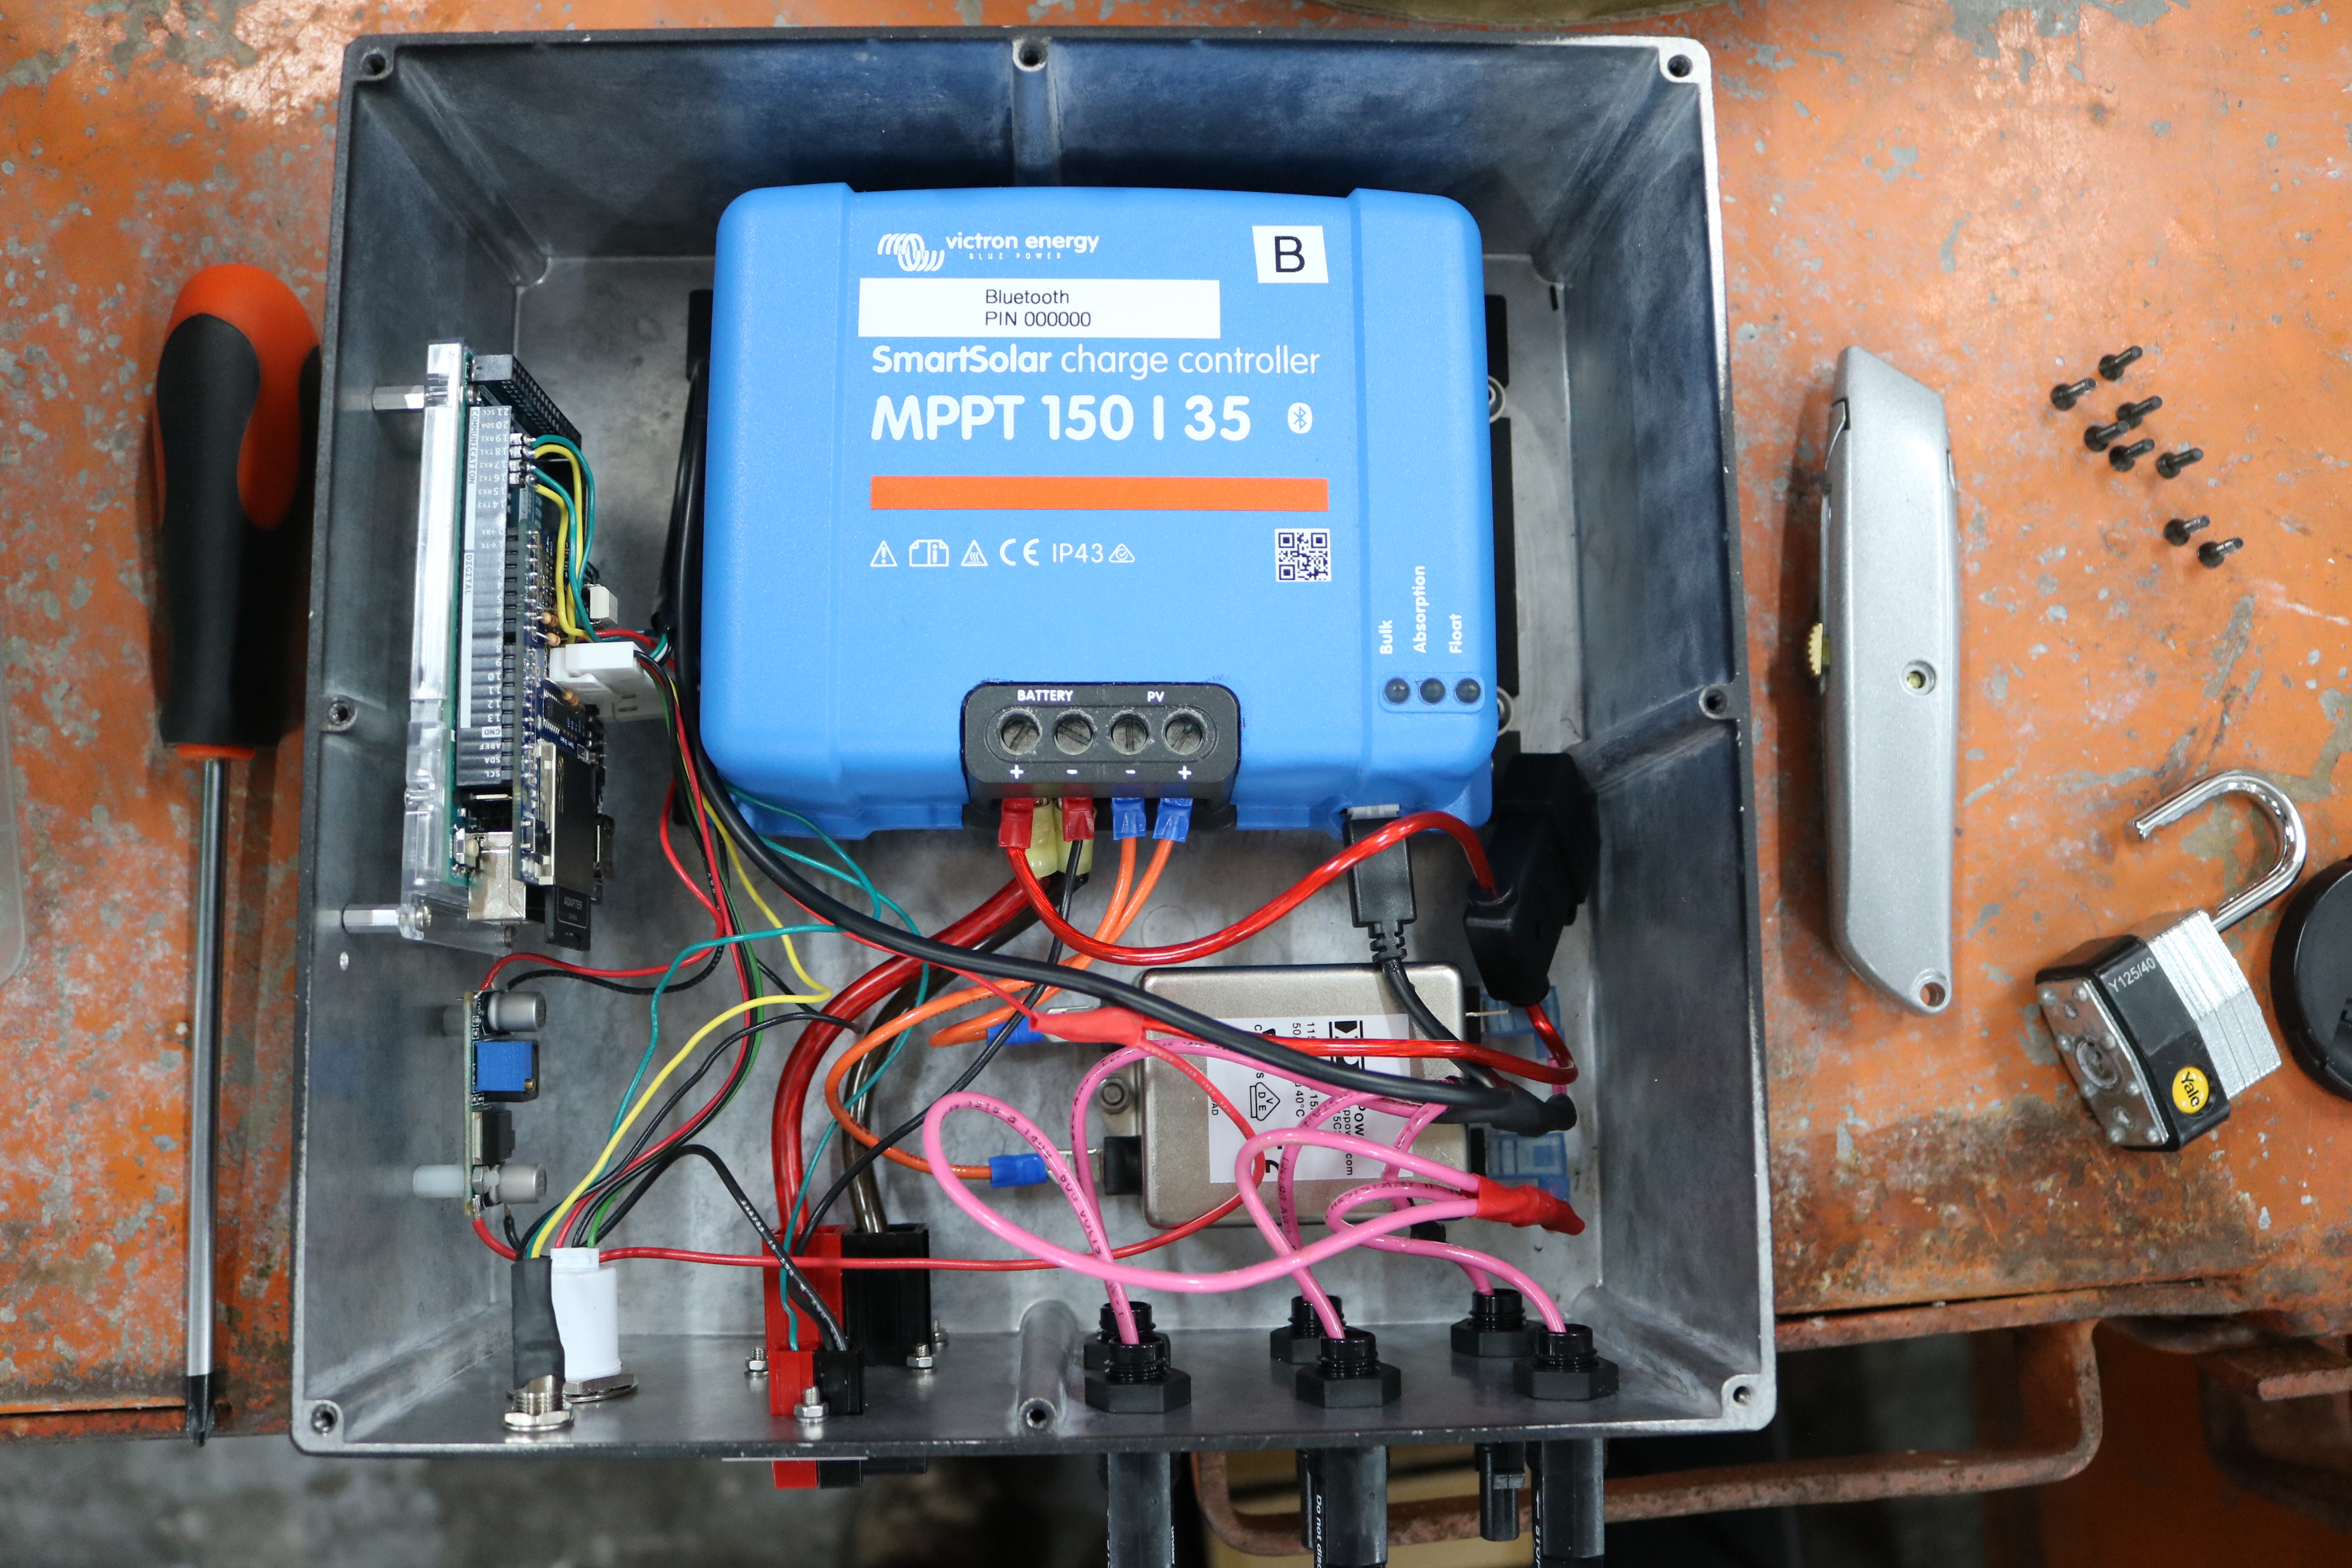
\includegraphics[width=\linewidth]{Figures/power_box_interior}
	\caption{The power logging and control system, the Victron charge controller, and an EMI filter are housed in an aluminum box.  \attention{[add relevant labels to the picture]}}
	\label{Fig:power_box_interior}
\end{figure}

\begin{figure}
	\centering
	\includegraphics[width=\linewidth]{Figures/station}
	\caption{April 2019 deployment of the first \albatros\ autonomous station was a success. The mounted solar panels and the LWA antenna are visible.  \attention{[Mention that the orange shipping container was only present temporarily during the takeover period when we were installing the hardware, but it's not part of the permanent installation.]}}
	\label{Fig:station}
\end{figure}

	\chapter{\prizm~Instrumentation}
    \section{\prizm~Experiment Overview}
    \section{Signal Chain}
        \subsection{}
        \subsection{}
        \subsection{}
    \section{Revised \prizm~Instrumentation}
        \subsection{}
          
        \subsection{}
	
	\chapter{Preliminary Data and Recommendations}

	
	\bibliographystyle{unsrtnat}   
	\bibliography{TH_Moso_MSc_Thesis}{}
	
\end{document}
